\section{Cast of Characters}




This difference between the plane and the sphere illustrates
the need to quantify how much a surface is curving.
What  do we require of a definition of curvature?
A straight line should have zero curvature and
 large circles should have less curvature than smaller circles.
We also need to differentiate between
curving to the left and curving to the right.

For any point on a smooth one dimensional curve in the plane,
we can approximate the curve with a circle.
The best approximating circle is the  \EMPH{osculating circle}.
A natural definition of the \EMPH{curvature} is the inverse of the radius of the osculating
 circle $k=\frac{1}{r}$.
See \figref{osculating-circle} for an example.
The osculating circle meets the requirements for a definition of curvature as long
as we allow the straight line to have an osculating circle with infinite radius.
We determine the sign of the curvature by which side of the curve the osculating circle is on.




The above definition provides great intuition for the curvature of curves
and surfaces.
Computing this value depends on how a curve or surface is represented. 

\begin{figure}[htb]
	\centering
	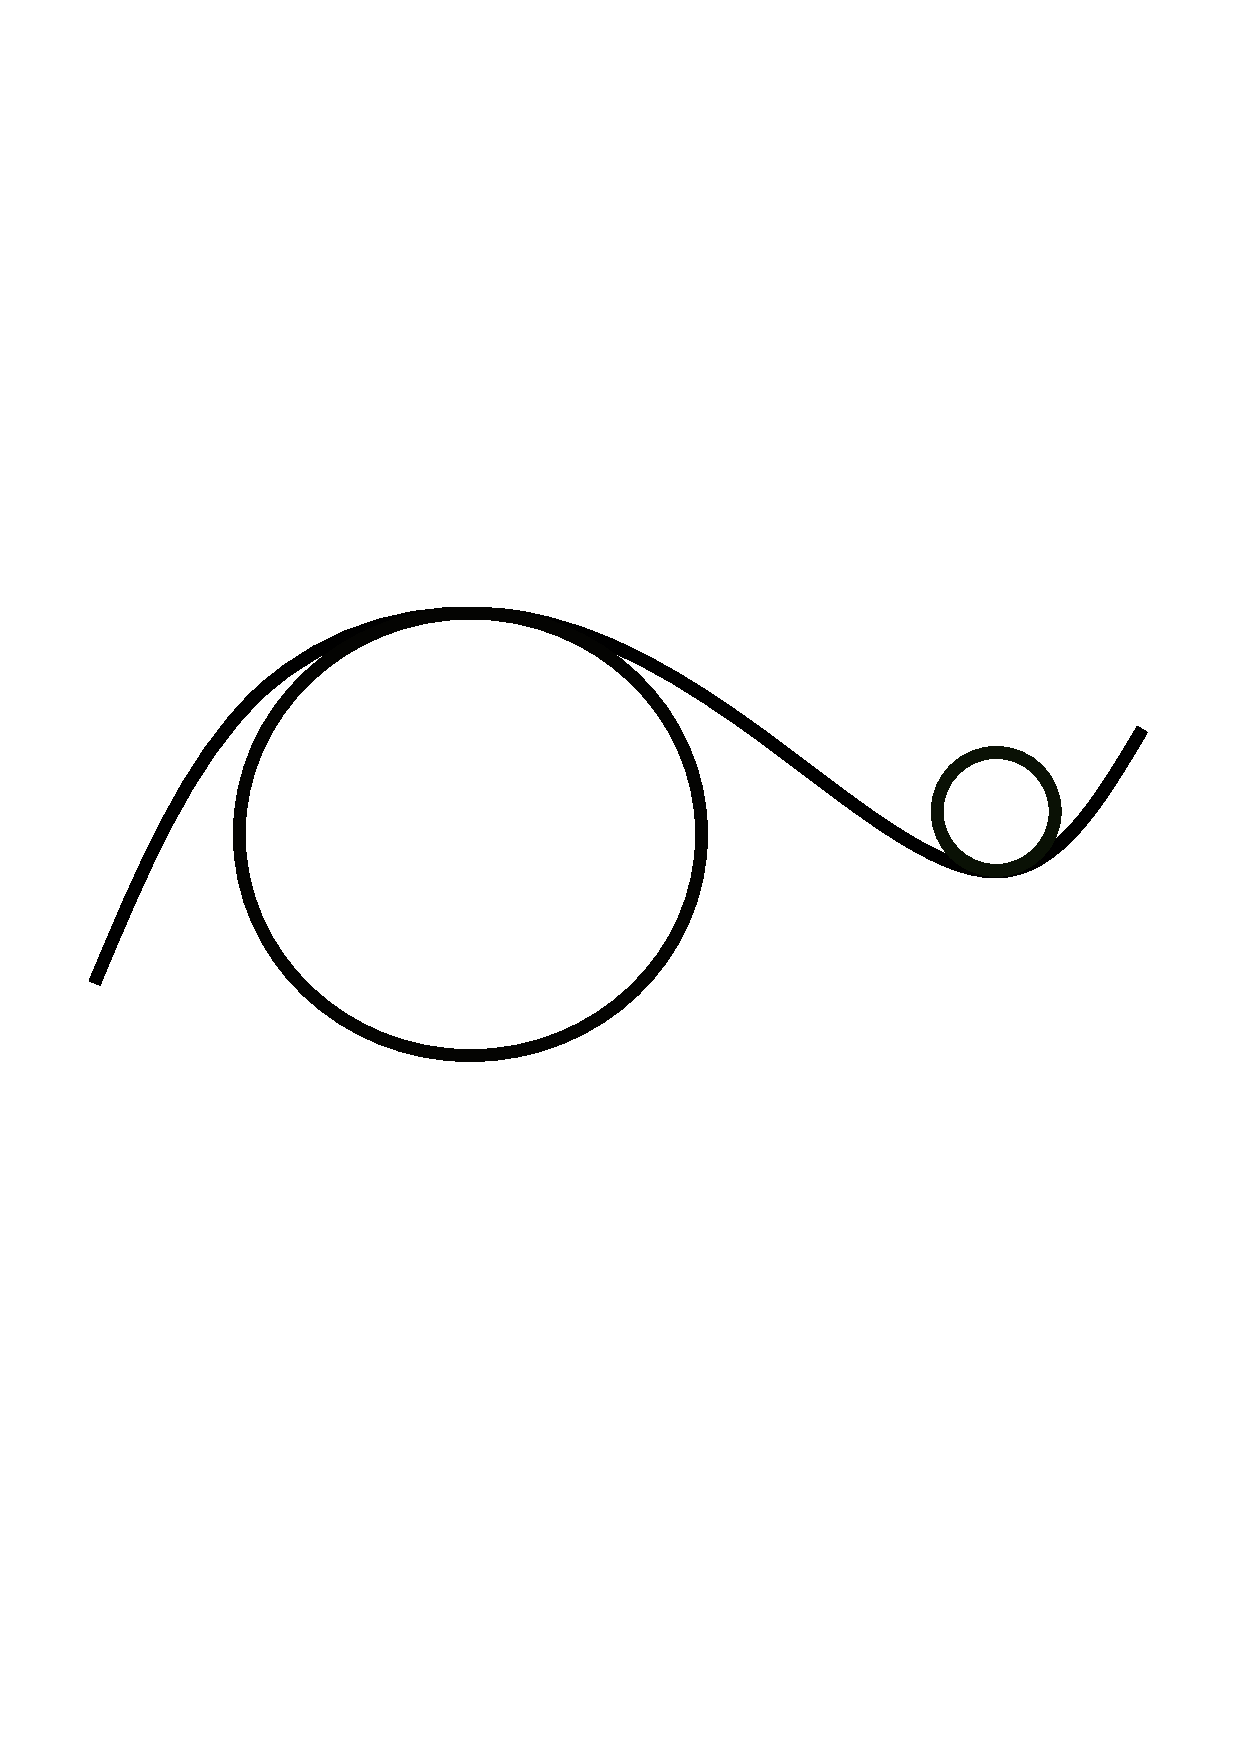
\includegraphics[width=.3\textwidth]{curvature/osculating}
	\caption{A curve with two osculating circles. The curvature at these points
	have opposite sign.}
	\label{fig:osculating-circle}
\end{figure}

A curve in $\RR^3$ is often presented as a function
$\gamma(t)=(x(t),y(t),z(t))$. We say that a curve is \EMPH{smooth} on an open interval $I$
if $\gamma'$ it is continuous and $\gamma'(t)\neq (0,0,0)$ on $I$. 
If $\gamma$ is smooth it has a well-defined unit tangent vector $T(t)=\frac{\gamma'(t)}{|\gamma'(t)|}.$
A second way to define the  \EMPH{curvature} at a point is as the signed magnitude of the rate of change of the 
unit tangent vector

\begin{equation} \label{eqn:kappa}
\kappa= \pm | T'(t)|.
\end{equation}
where $t$ is arc length.

For example, take a circle of radius $r$, parameterized by 
$$C(t)=\left(r\cos(t),r\sin(t),0\right).$$
We have 
$$\frac{dC}{dt}=C'(t)=\left(-r\sin(t),r\cos(t),0\right)$$ and $|C'(t)|=r.$
Then $T(t)=\left(-\sin(t),\cos(t),0\right)$ and
$T'(t)=\left(-\cos(t),-\sin(t),0\right)$.
So, $\kappa(t)=\frac{1}{r}$ and, in this case, our definition of curvature agrees with the
osculating circle intuition given above. 
\eqnref{kappa} can be rewritten in the following more computational friendly form 
\begin{equation} \label{eqn:kappa1}
\kappa(t)=\frac{|\gamma'(t)\times \gamma''(t)|}{|\gamma'(t)|^3}.
\end{equation}

We traverse $\gamma$
at unit speed so that the length of the velocity vector is one, $\gamma'(t)^2=1,$ and by the chain rule, $\gamma'\cdot \gamma''=0$.
This implies $\gamma'$ and $\gamma''$ are orthogonal.
Thus, the
vector $\gamma''=N$ is normal to the $\gamma$. 
By taking the cross product of $N$ and $T$ we obtain a vector $B$ called
the binormal vector.
%The vectors $T,N$ and $B$ form the \EMPH{Fernet frame} of $\gamma$ a $p.$

 This osculating-circle idea can be extend
to  surfaces in $\R^3$, by considering the \EMPH{osculating sphere},
But notice that at saddle points on a surface it is not clear which sphere
best approximates the surface. See \figref{osculating-sphere} for two
equally reasonable ways to approximate a saddle with a sphere.

\begin{figure}[htb]
    \captionsetup[subfigure]{justification=centering}
    \centering
    \begin{subfigure}[b]{0.25\textwidth}
        \includegraphics[width=\textwidth]{curvature/sphere-above-saddle}
       \subcaption{}\label{fig:sphere-above-saddle}
    \end{subfigure}
        \hspace{1cm}
        \begin{subfigure}[b]{0.25\textwidth}
        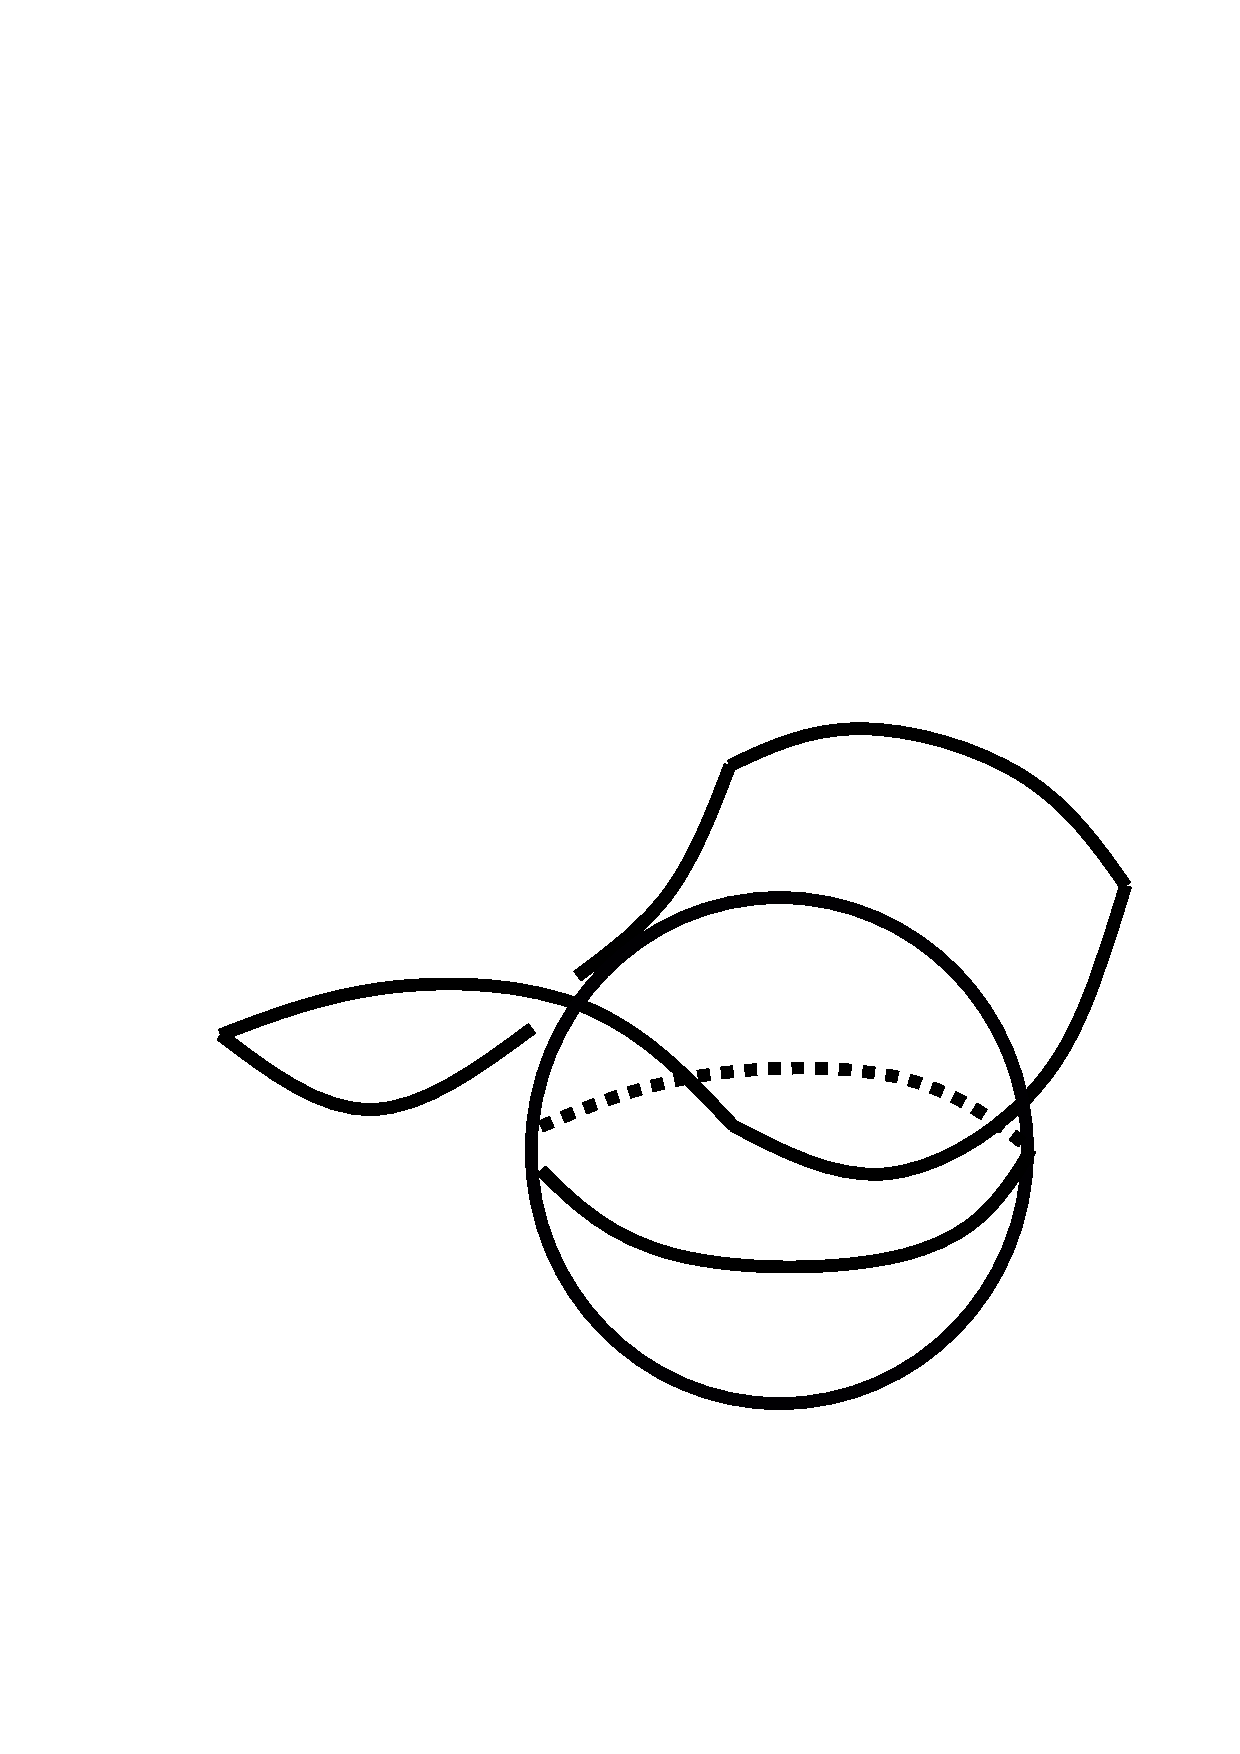
\includegraphics[width=\textwidth]{curvature/sphere-below-saddle}
        \subcaption{}\label{fig:sphere-below-saddle}
        \end{subfigure}
    \caption{(\subref{fig:sphere-above-saddle}) The osculating sphere above the saddle.
        (\subref{fig:sphere-below-saddle}) The osculating sphere above the saddle.
    }
    \label{fig:osculating-sphere}
\end{figure}



\subsection{Gaussian Curvature}


One dimensional curves are represented by differentiable 
parameterized functions $\gamma:I\subset \RR\to \RR^3$,
we would now like to parameterize a surface.
Similarly, a \EMPH{parameterized surface} $S$ is a collection of maps such that
 for each point $p\in S$ we have a neighborhood $X\subset S$
 and a map $r:U\subset \RR^2 \to X\subset \RR^3$, $r(u,v)=(x(u,v),y(u,v),z(u,v))$
 where
 \begin{itemize}
 \item  $r$ is a homeomorphism
 \item $r$ has derivatives of all orders
 \item every point in $S$ is contained in the domain of at least one map.

\end{itemize}
The maps in the third item are called \EMPH{charts}.
If the differential $dr_q:\RR^2\to \RR^3$ is one-to-one for all $q\in U$ then
we say $r$ is \EMPH{regular}. In other words, let $(u,v)$ be coordinates of $U\subset \RR^2,$
a surface is regular if $\frac{\partial r}{\partial u}$
and $\frac{\partial r}{\partial v}$ are linearly independent for all $p\in U$.
Once we choose a chart we define a clockwise orientation to be positive.
 If the clockwise orientation can be consistently extended to the entire surface, we say
the surface is \EMPH{orientable}.


\begin{example}[The Sphere]\label{ex:sphere-charts}

The unit two sphere $\Sp^2\subset \RR^3$ is the set $\{(x,y,z)\in \RR^3 | x^2+y^2+z^2=1\}.$
We can define six charts to parameterize $\Sp^2$.
For $u,v\in[-1,1]$, we have
$$r_{z}(u,v)=(u,v,\sqrt{1-u^2-v^2}) \hspace{.5cm}  r_{-z}(u,v)=(u,v,-\sqrt{1-u^2-v^2}) \hspace{.5cm}  r_{x}(u,v)=(\sqrt{1-u^2-v^2},u,v) $$
$$r_{-x}(u,v)=(-\sqrt{1-u^2-v^2},u,v) \hspace{.5cm}  r_{y}(u,v)=(u,\sqrt{1-u^2-v^2},v) \hspace{.5cm}   r_{-y}(u,v)=(u,-\sqrt{1-u^2-v^2},v). $$

The chart $r_{z}$ is shown in \figref{sphere-chart}

\begin{figure}[htb]
	\centering
	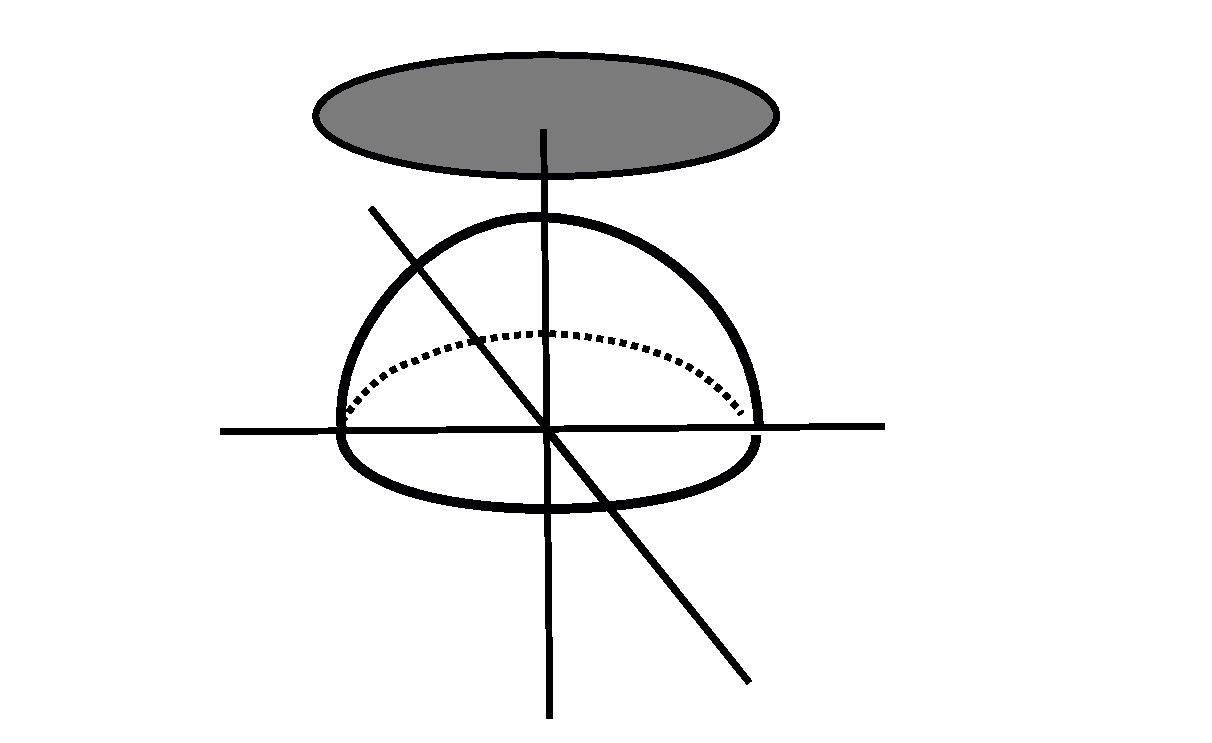
\includegraphics[width=.4\textwidth]{curvature/sphere-chart}
	\caption{A chart of $\Sp^2$.}
	\label{fig:sphere-chart}
\end{figure}

One can verify that these parameterizations fulfill the requirements
for the sphere to be a regular surface.

\end{example}


A \EMPH{tangent vector} to $S$ at $p$ is a map $\xi:(-\epsilon,\epsilon)\to S$ with $\xi(0)=p$.
The set of all tangent vectors is the \EMPH{tangent plane} and it corresponds to the image
of the differential map $d\phi_q(\RR^2)\subset \RR^3$ (prop. 1 \cite{doc76}).
By choosing two linearly independent paths through $p\in S$ we obtain a basis 
for the tangent
plane and define a normal vector $N$ at $p$.
Every plane containing the normal vector will intersect the surface.
The intersection of the surface and each normal plane is a curve in $\RR^3$
gives a one dimensional curve called the \EMPH{normal section}, see  \figref{normal-sections}
for an example.
Let $\kappa_1$ denote the maximum curvature of all normal sections 
and let $\kappa_2$ denote the minimum. 
The \EMPH{Gaussian curvature} of a point on a surface is
$K=\kappa_1\kappa_2.$
One can check that the Gaussian curvature of the plane is zero and
that larger circles have less curvature than smaller ones.



\begin{figure}[htb]
    \captionsetup[subfigure]{justification=centering}
    \centering
    \begin{subfigure}[b]{0.25\textwidth}
        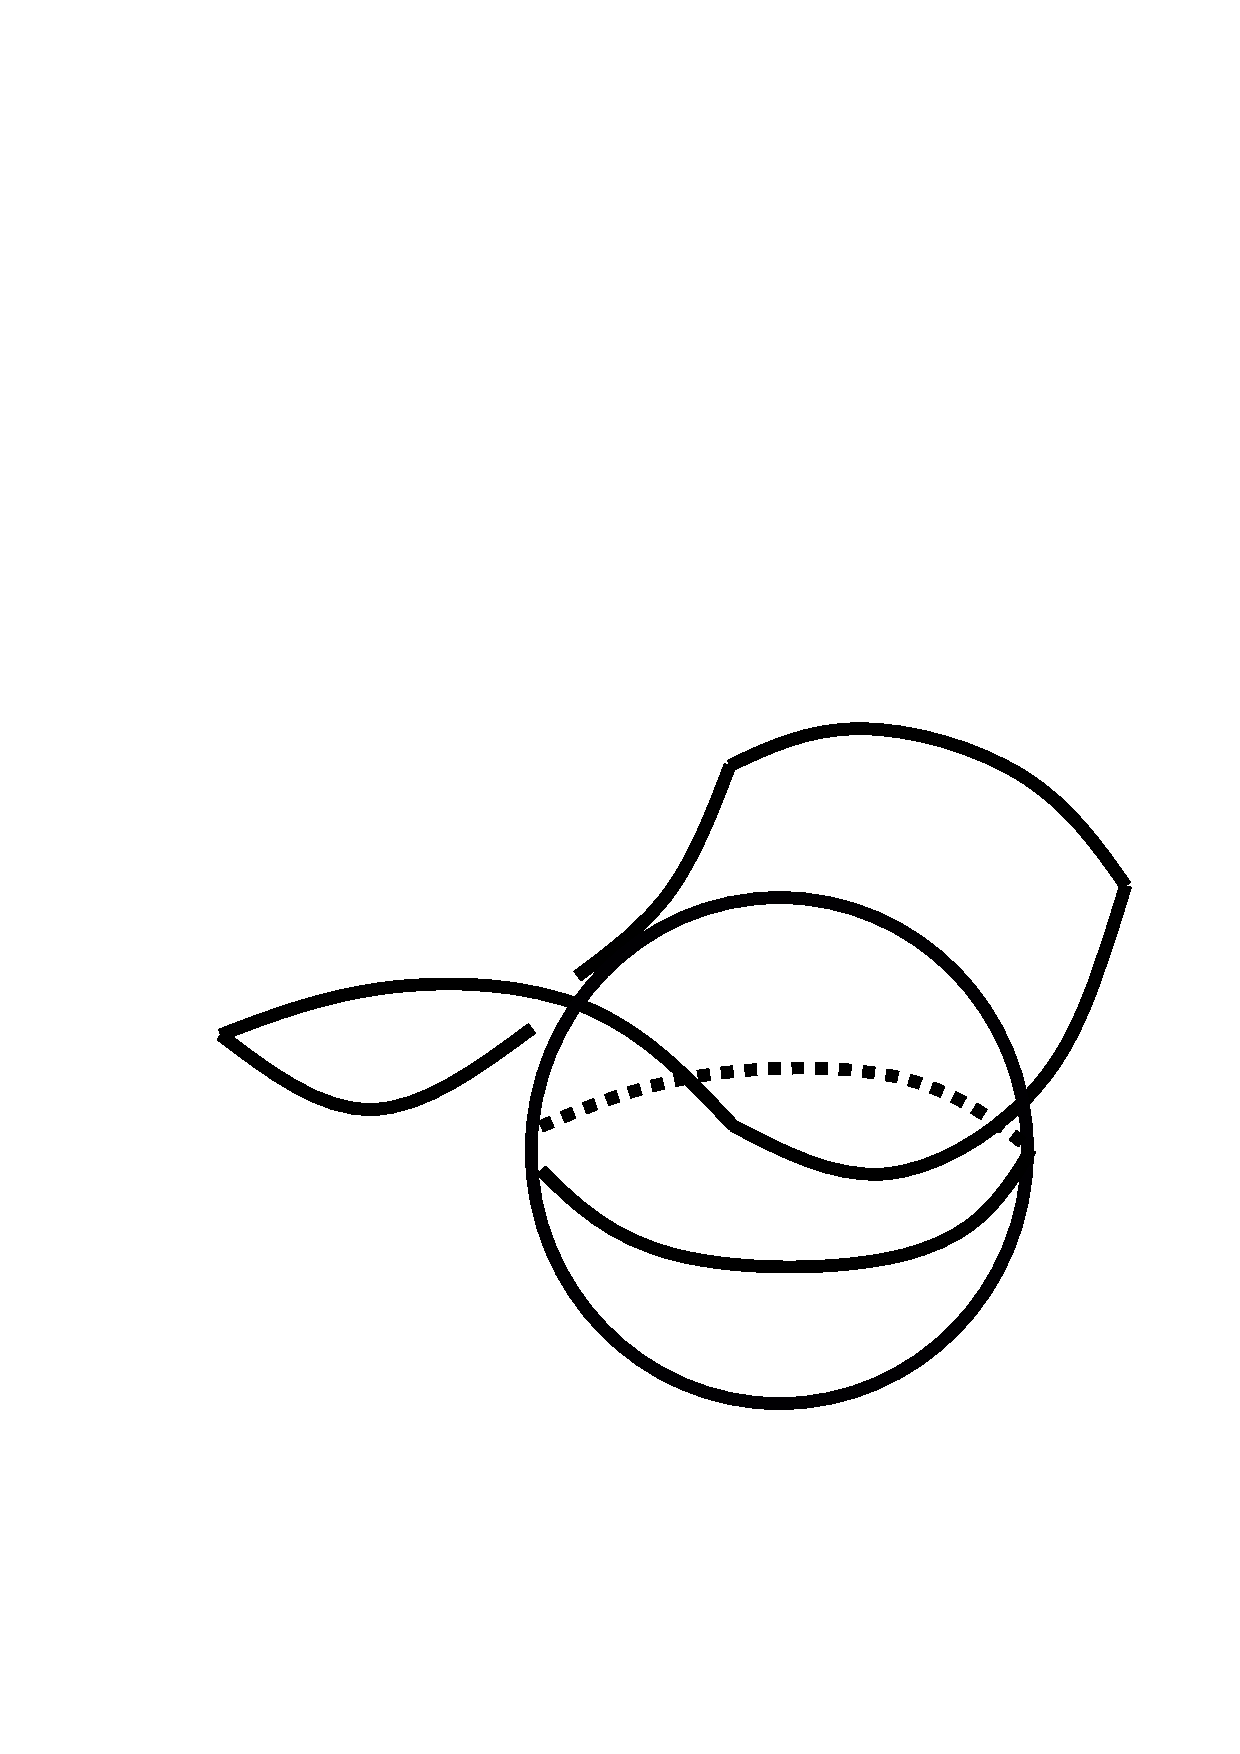
\includegraphics[width=\textwidth]{curvature/normal-section-max}
       \subcaption{}\label{fig:normal-section-max}
    \end{subfigure}
        \hspace{1cm}
        \begin{subfigure}[b]{0.25\textwidth}
        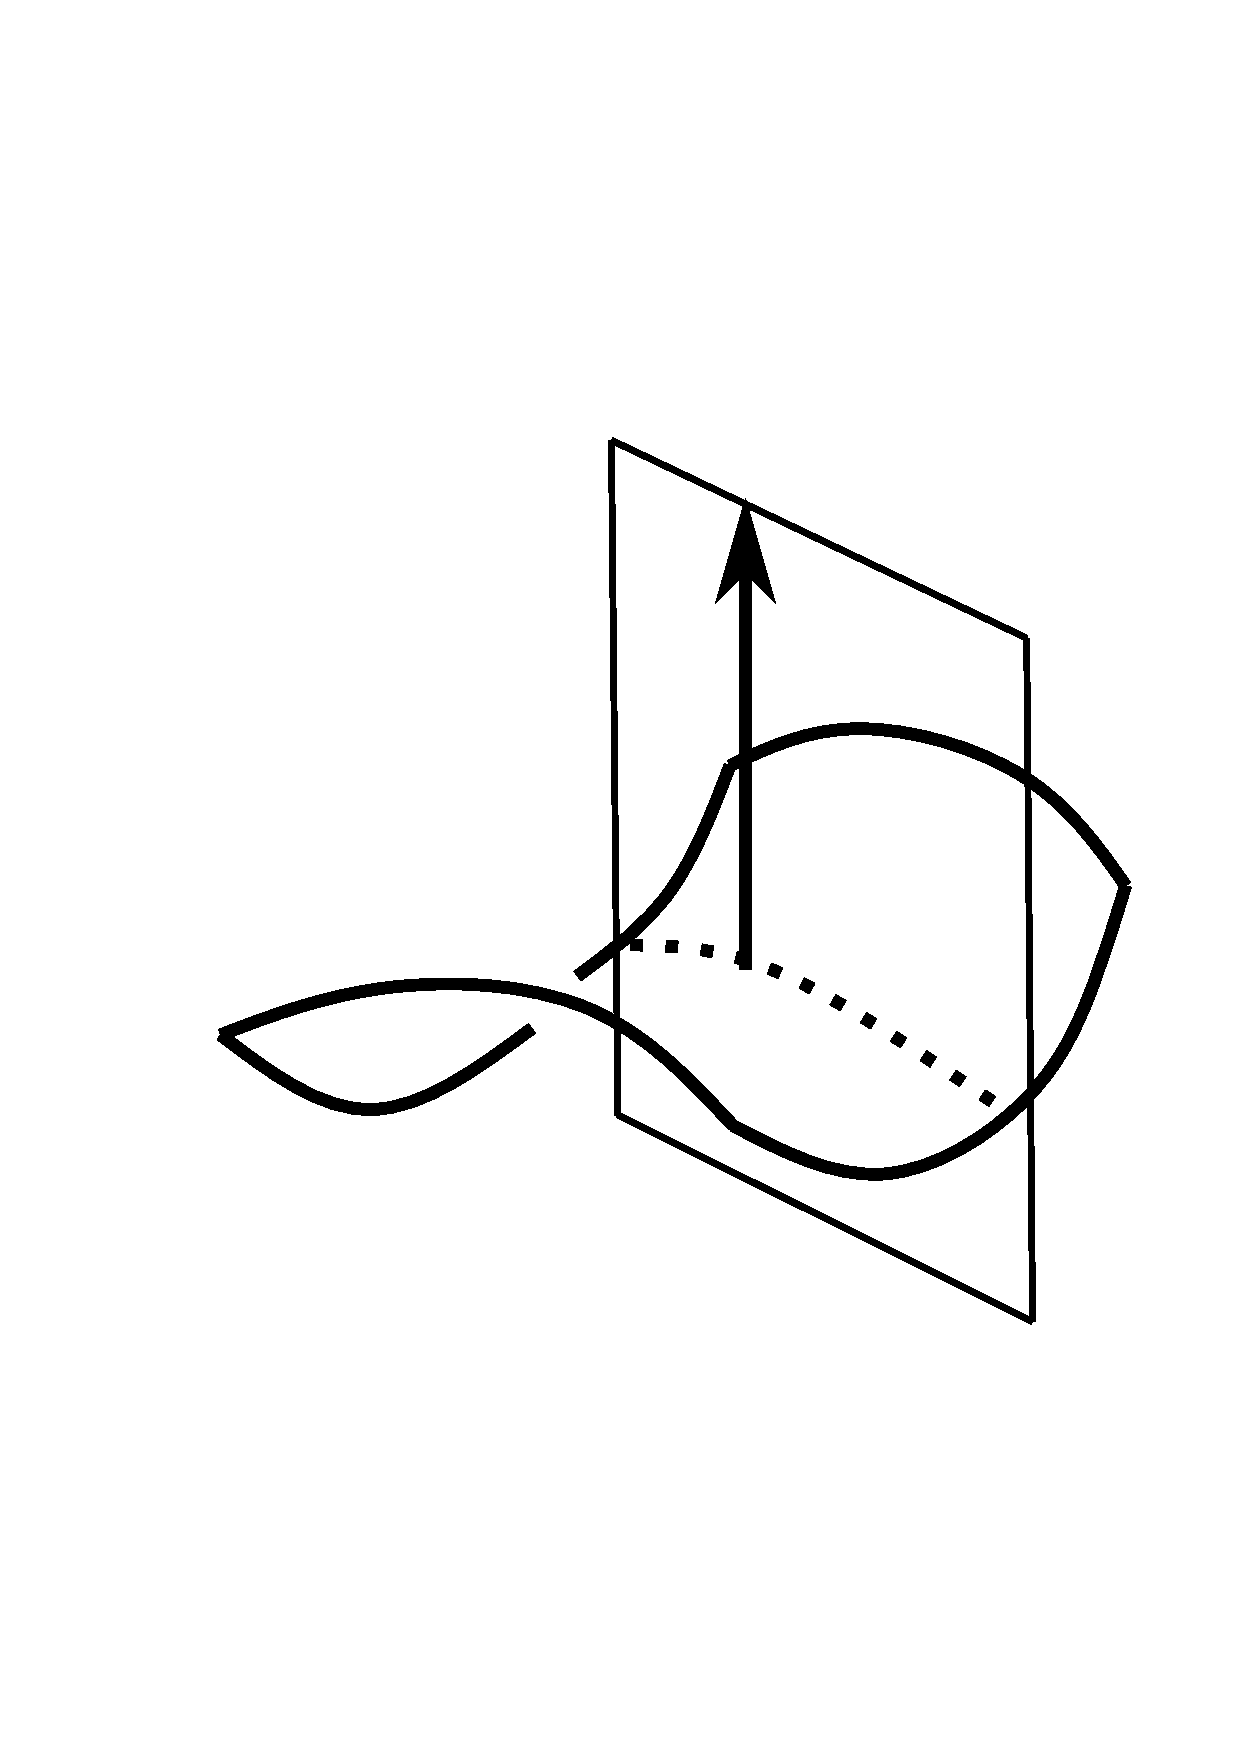
\includegraphics[width=\textwidth]{curvature/normal-section-min}
        \subcaption{}\label{fig:normal-section-min}
        \end{subfigure}
    \caption{(\subref{fig:normal-section-max}) The osculating sphere above the saddle.
        (\subref{fig:normal-section-min}) The osculating sphere above the saddle.
    }
    \label{fig:normal-sections}
\end{figure}


We now consider computing the Gaussian curvature.
A \EMPH{quadratic form} to be polynomial of degree two, of the form $p(u,v)=c_1u^2+c_2uv+c_3v^2$ 
where $c_i\in R$.
We define a quadratic form, the first fundamental form, using $r(u,v)$.

Let $r(u,v)$ be a parameterized surface.
Let $E=r_u\cdot r_u, F=r_u\cdot r_v$ and  $G=r_v\cdot r_v$.
The \EMPH{first fundamental form}
is the quadratic form $\mathrm{I}=Edu^2+2Fdudv +Gdv^2$.
We summarize the first fundamental form as a matrix $$\mathrm{I}=\begin{bmatrix}
E & F \\
F & G 
\end{bmatrix}.$$
%We get a notion of length in the tangent space, an inner product on $Tp(S)$.
%If $x$ and $y$ are two tangent vectors
%then $$\mathrm{I}(x,y)=x^T\begin{bmatrix}
%E & F \\
%F & G 
%\end{bmatrix}y.$$

The first fundamental form enables us to  compute many interesting
things about our surface including arc length, angles between curves,
and area on a surface.
For example,
given a `small' parallelogram $M$ on $S$ with corners $r(u,v),r(u+\epsilon u, v), r(u,v+\epsilon v)$ 
and $r(u+\epsilon u, v+\epsilon v)$ the rate of change of the area of $M$ is 
$$dA=\sqrt{EG-F^2}dudv.$$
In \exref{stereo}, we will use the first fundamental form to compute the arc length of some curves.


Gauss's Egregious (remarkable) Theorem states that the Gaussian curvature only depends
of the first fundamental form. Thus, curvature can be computed entirely by measuring angles, distance 
and their derivatives without any reference to the way that the surface is embedded in $\R^3.$
Because of this property we say that Gaussian curvature is an \emph{intrinsic} property of a surface.
The Brioschi formula gives the Gaussian curvature using only the first fundamental form
\begin{equation}\label{eq:brioschi}
	K=\frac{\begin{vmatrix}
-\frac{1}{2}E_{vv}+F_{uv}-\frac{1}{2}G_{uu} & \frac{1}{2}E_u & F_u-\frac{1}{2}E_v\\
F_v-\frac{1}{2}G_u & E & F\\
\frac{1}{2}G_v & F & G
\end{vmatrix}-\begin{vmatrix}
0 & \frac{1}{2}E_v & \frac{1}{2}G_u\\
\frac{1}{2}E_v & E & F\\
\frac{1}{2}G_u & F & G
\end{vmatrix}}{(EG-F^2)^2}
\end{equation}



While we can compute Gaussian curvature using only the first fundamental form,
 the second fundamental form is convenient for computations.
To this end, the unit normal vector at $p$ is given by $$n(p)=\frac{r_u\times r_v}{|r_u\times r_v|}.$$
Let $L=r_{uu}\cdot n, M=r_{uv}\cdot n$ and $N=r_{vv}\cdot n$ the
\EMPH{second fundamental form} is $\mathrm{I\!I}=Ldu^2+2Mdudv+Ndv^2$,
in matrix form $$\mathrm{I\!I}=\begin{bmatrix}
L & M \\
M & N 
\end{bmatrix}.$$
%Another inner product is given by $$\mathrm{I\!I}(x,y)=x^T\begin{bmatrix}
%L & M \\
%M & N 
%\end{bmatrix}y.$$
Combining the first and second fundamental forms we have
the \EMPH{Gaussian curvature} of a surface is
\begin{equation}\label{eqn:curve-dets}
 	K=\frac{\det(\mathrm{I\!I})}{\det(\mathrm{I})}.
\end{equation}

\begin{example}[Curvature of the Sphere]\label{ex:compute-surface-curvature}
Consider the northern hemisphere of the unit sphere parameterized
by $$r(u,v)=(u,v,\sqrt{1-u^2-v^2})$$ and we wish to compute the Gaussian curvature at
the north pole $p=(0,0,1)$.
We have $$r_u|_p=(1,0,\frac{-u}{\sqrt{1-u^2-v^2}})|_p=(1,0,0)$$ and
$$r_v|_p=(0,1,\frac{-v}{\sqrt{1-u^2-v^2}})|_p=(0,1,0).$$
We have $E=1, F=0,$ and $G=1$ so our first fundamental form is
$\mathrm{I}=\begin{bmatrix}
1 & 0 \\
0 & 1 
\end{bmatrix}.$
Our normal vector is $n(p)=(0,0,1)$ with 
$$r_{uu}|_p=(0,0,\frac{1-2u^2}{(1-u^2)^{\frac{3}{2}})})|_p=(0,0,1),
r_{uv}|_p=(0,0,0)$$ and 
$$r_{vv}|_p=(0,0,\frac{1-2v^2}{(1-v^2)^{\frac{3}{2}})})|_p=(0,0,1).$$
Thus, $L=1, M=0$ and $N=1$ and our second fundamental form is
$\mathrm{I\!I}=\begin{bmatrix}
1 & 0 \\
0 & 1 
\end{bmatrix}$
and our Gaussian curvature is $K=\frac{\det(\mathrm{I\!I})}{\det(\mathrm{I})}=\frac{1}{1}=1$ as expected.

\end{example}

We will use the first fundamental form to compute
the arc length of circles on the sphere parallel to the $xy$ plane with fixed height $z=c$ for $-1<c<1$.
Stereographic projection, described in \secref{plane-sphere},
allows us map our problem to the plane and perform our computations there.

\begin{example}[Stereographic Projection Revisited\cite{christian-notes}]\label{ex:stereo}
Consider the two sphere with the north pole removed $\Sp^2 \setminus (0,0,1)$,
stereographic projection is a bijection between the points on $\Sp^2 \setminus (0,0,1)$ to the $\R^2$.
Consider a line from the north pole $(0,0,1)$ that intersects $(x,y,z)\in \Sp^2$ parametrized by 
$p(t)=(1-t)(0,0,1)+t(x,y,z)$. By considering the $z$ coordinate we determine the $t$ value where this line
intersects $\R^2$, namely $t=\frac{1}{1-z}.$
This gives the desired map shown in \figref{stereo} and in equation form
$$p(x,y,z)\to \left(\frac{x}{1-z},\frac{y}{1-z}\right).$$

\begin{figure}[htb]
	\centering
	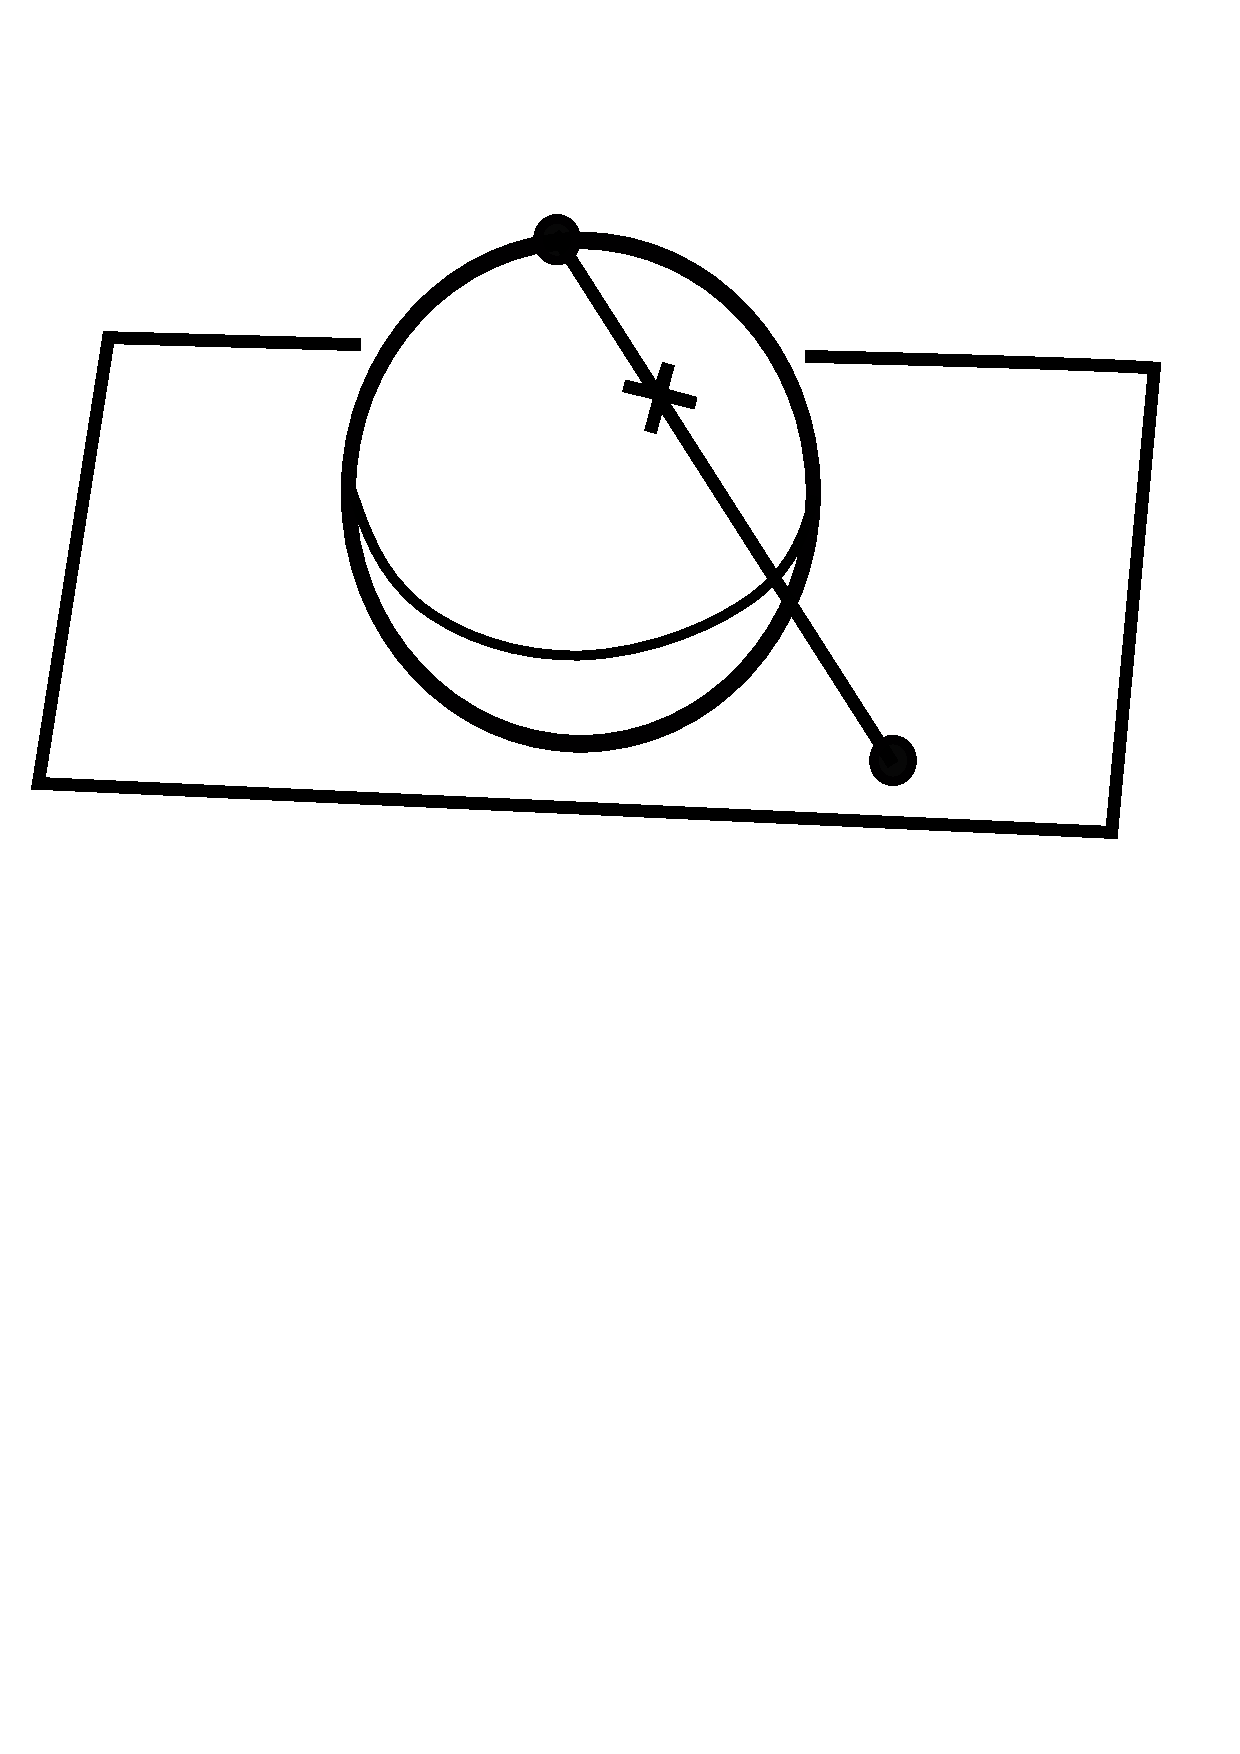
\includegraphics[width=.3\textwidth]{curvature/stereo}
	\caption{A point on the sphere is mapped to a point on the plane by stereographic projection.}
	\label{fig:stereo}
\end{figure}
	
The inverse is given by $p^{-1}:\R^2\to \R^3$

	\begin{equation}\label{eqn:stereo}
		p^{-1}(u,v)=\left(\frac{2u}{u^2+v^2+1},\frac{2v}{u^2+v^2+1},\frac{u^2+v^2-1}{u^2+v^2+1}\right).	
	\end{equation}
To compute the first fundamental form of $p^{-1}(u,v)$ we take the partial derivatives

$$p^{-1}_u=\left(\frac{2v^2-2u^2+2}{(u^2+v^2+1)^2},\frac{-4uv}{(u^2+v^2+1)^2},\frac{4v}{(u^2+v^2+1)^2}\right)$$
and 
$$p^{-1}_v=\left(\frac{-4uv}{(u^2+v^2+1)^2},\frac{2v^2-2u^2+2}{(u^2+v^2+1)^2},\frac{4v}{(u^2+v^2+1)^2}\right).$$
Then, after some algebra,
$$E=p^{-1}_u\cdot p^{-1}_u=\frac{4}{(u^2+v^2+1)^2}$$
$$F=p^{-1}_v\cdot p^{-1}_v=\frac{4}{(u^2+v^2+1)^2}$$
and
$$M=p^{-1}_u\cdot p^{-1}_v=0.$$

We can use the first fundamental form to compute
the arc length of circles on the sphere parallel to the $xy$ plane with fixed height $z=c$ for $-1<c<1$.
This length can be computed using
the pythagorean theorem. We will see that using stereographic projection
and the first fundamental form we get the same answer.


The arc length of a parameterized curve $u=u(t), v=v(t)$ on a regular surface,
can be computed using the first fundamental form.  Let
$s$ denote the arc length, then 
$$ds=\bigg | \frac{dr}{dt}\bigg | dt = \bigg | r_u\frac{du}{dt}+r_v\frac{dv}{dt}\bigg |dt
=\sqrt{(r_u^2 du^2+2r_ur_v du dv + r_v^2dv^2)}.$$
Next, use the map $p$ to map such a circle to the plane.
Using \eqnref{stereo}, our circle on the sphere maps 
to a circle in the plane because
	$$p^{-1}(u,v)=\frac{u^2+v^2-1}{u^2+v^2+1}=c$$
and we can compute the radius in terms of $c$
\begin{equation}\label{eqn:radius}
	u^2+v^2=\frac{1+c}{1-c}=k^2.
\end{equation}
	
In the plane, $u^2+v^2=k^2$ can be parameterized
as $$\gamma(t)=(k\cos(t),k\sin(t))$$ with $0\leq t\leq 2\pi.$
So our curve becomes $p^{-1}\circ \gamma(t)$ on the sphere.
Computing the partial derivatives of $\gamma(t)$ gives
$$\gamma_u'=-k\sin(t)\hspace{1.3cm}  \gamma_v'=k\cos(t).$$
Now we use the first fundamental form

$$\int_{p^{-1}}\gamma ds=\int_{0}^{2\pi} ||(p^{-1}\circ \gamma)'(t)dt=\int_0^{2\pi}\sqrt{E(\gamma_u'(t))^2+2M\gamma_u'\gamma_v'+
F(\gamma_v'(t))^2}dt.$$
Substituting and simplifying using $E=F$ we obtain
$$\int_0^{2\pi}\frac{2k}{k^2+1}dt=\frac{4\pi k}{k^2+1}.$$
Simplifying further using \eqnref{radius}  our arc length is
$$2\pi\sqrt{1-c^2}.$$

\end{example}

Stereographic projection has the property that it preserves the angles.
Maps with this property have a name.
\begin{definition}[Conformal]\label{def:conformal}
	Let $U$ and $V$ be open subsets of $\R^n$, a function $f:U\to V$ is
	\emph{conformal} at a point $u\in U$ if it preserves angles between curves
	through $u$ and preserves orientation.
\end{definition}
Proof that stereographic projection is conformal and circle preserving \cite{hilbert-imagination}.

\begin{theorem}[First Fundamental Form and Conformal Maps]\label{thm:first-conformal}
	Let $S$ be a regular surface and $f:U\subset \R^2 \to V\subset S$ be a chart.
	Let $f$ have first fundamental form $\mathrm{I}=Edu^2+2Fdudv +Gdv^2$.
	Then $f$ is conformal if and only if $E=G$ and $F=0.$
\end{theorem}


\subsection{Geodesics Curvature}

Shortest paths play an important role in many computational problems.
On a surface, a \EMPH{geodesic} is a curve that is a shortest path
between two points in the surface. 
For example, on $\Sp^2$ great circles are geodesic.
Intuitively, the geodesic curvature of a one dimensional curve on a surface
is the curvature as it would be seen from someone living on the surface.


Given a parameterized surface and a point on parameterized curve on the surface,
we can compute the geodesic curvature as follows.
First, find the tangent plane to the surface at the point and the unit normal vector.
Let $U:\mathcal{U}\to \RR^3$ be a parameterized chart on a surface $S$ with vector $n(u,v)$ normal
to the surface
and let $\gamma(\theta)$ be a curve in $U$.
Then $V=n(\gamma(\theta))\times T$ is in the tangent plane of the surface since
it is perpendicular to $n$. Moreover, $V(\theta)$ is normal to $\gamma$ 
from the perspective of someone living on the surface. 
The geodesic curvature tells us the rate of change of $\gamma'$ with respect 
to $V(\theta)$.
The \EMPH{geodesic curvature} is given by 
\begin{equation} \label{eqn:geodesic}
	k_g=\gamma'' \cdot (V\times \gamma').
\end{equation}

\begin{example}[Circles on the Sphere]\label{eqn:circles-on-sphere}
	We can rotate the sphere so that the circle is parallel to the $xy$-plane.
	Then the radius of the circle $r$ is related to the height $h$ of the circle above the $xy$-plane
	by $h^2+r^2=1$. See \figref{geodesic} for an example.
	A parameterization by arc length is given by
	$$\gamma(\theta)=\left(r\cos\left(\frac{\theta}{r}\right),r\sin\left(\frac{\theta}{r}\right),\sqrt{1-r^2}\right),$$
	so
	$$\gamma'(\theta)=\left(-\sin\left(\frac{\theta}{r}\right),\cos\left(\frac{\theta}{r}\right),0\right)$$
	and
	$$\gamma''(\theta)=\left(-\frac{1}{r}\cos\left(\frac{\theta}{r}\right),-\frac{1}{r}\sin\left(\frac{\theta}{r}\right),0\right).$$
	Since we are on the sphere, the normal vector is equal to the point on the sphere
	so $$n(\theta)=\left(r\cos\left(\frac{\theta}{r}\right),r\sin\left(\frac{\theta}{r}\right),\sqrt{1-r^2}\right).$$
	Then 
	$$k_g=\gamma''\cdot V(\theta)=\frac{\sqrt{1-r^2}}{r}.$$
	Notice that if $h=0$ then $r=1$ and the geodesic curvature is zero on the equator.
\end{example}

\begin{figure}[htb]
	\centering
	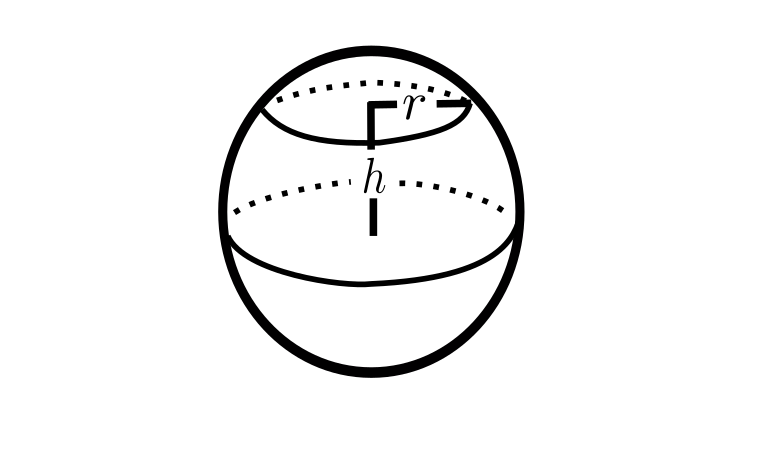
\includegraphics[width=.25\textwidth]{curvature/geodesic}
	\caption{Computing the geodesic curvature.}
	\label{fig:geodesic}
\end{figure}


\subsection{Triangulations and The Euler Characteristic}

We assume the reader is familiar with the notions
of topological spaces and simplicial complexes.
Most introductory topology texts describe these objects \cite{jm08,munkres}.
The applications we will encounter will refer to triangulated surfaces in $\R^3$
called a \EMPH{mesh}, in one application the surface will contain its interior.
Each triangle in a mesh is isomorphic to a triangle in the plane and the sum
of the interior angles is $\pi$.









\begin{figure}[htb]
\centering
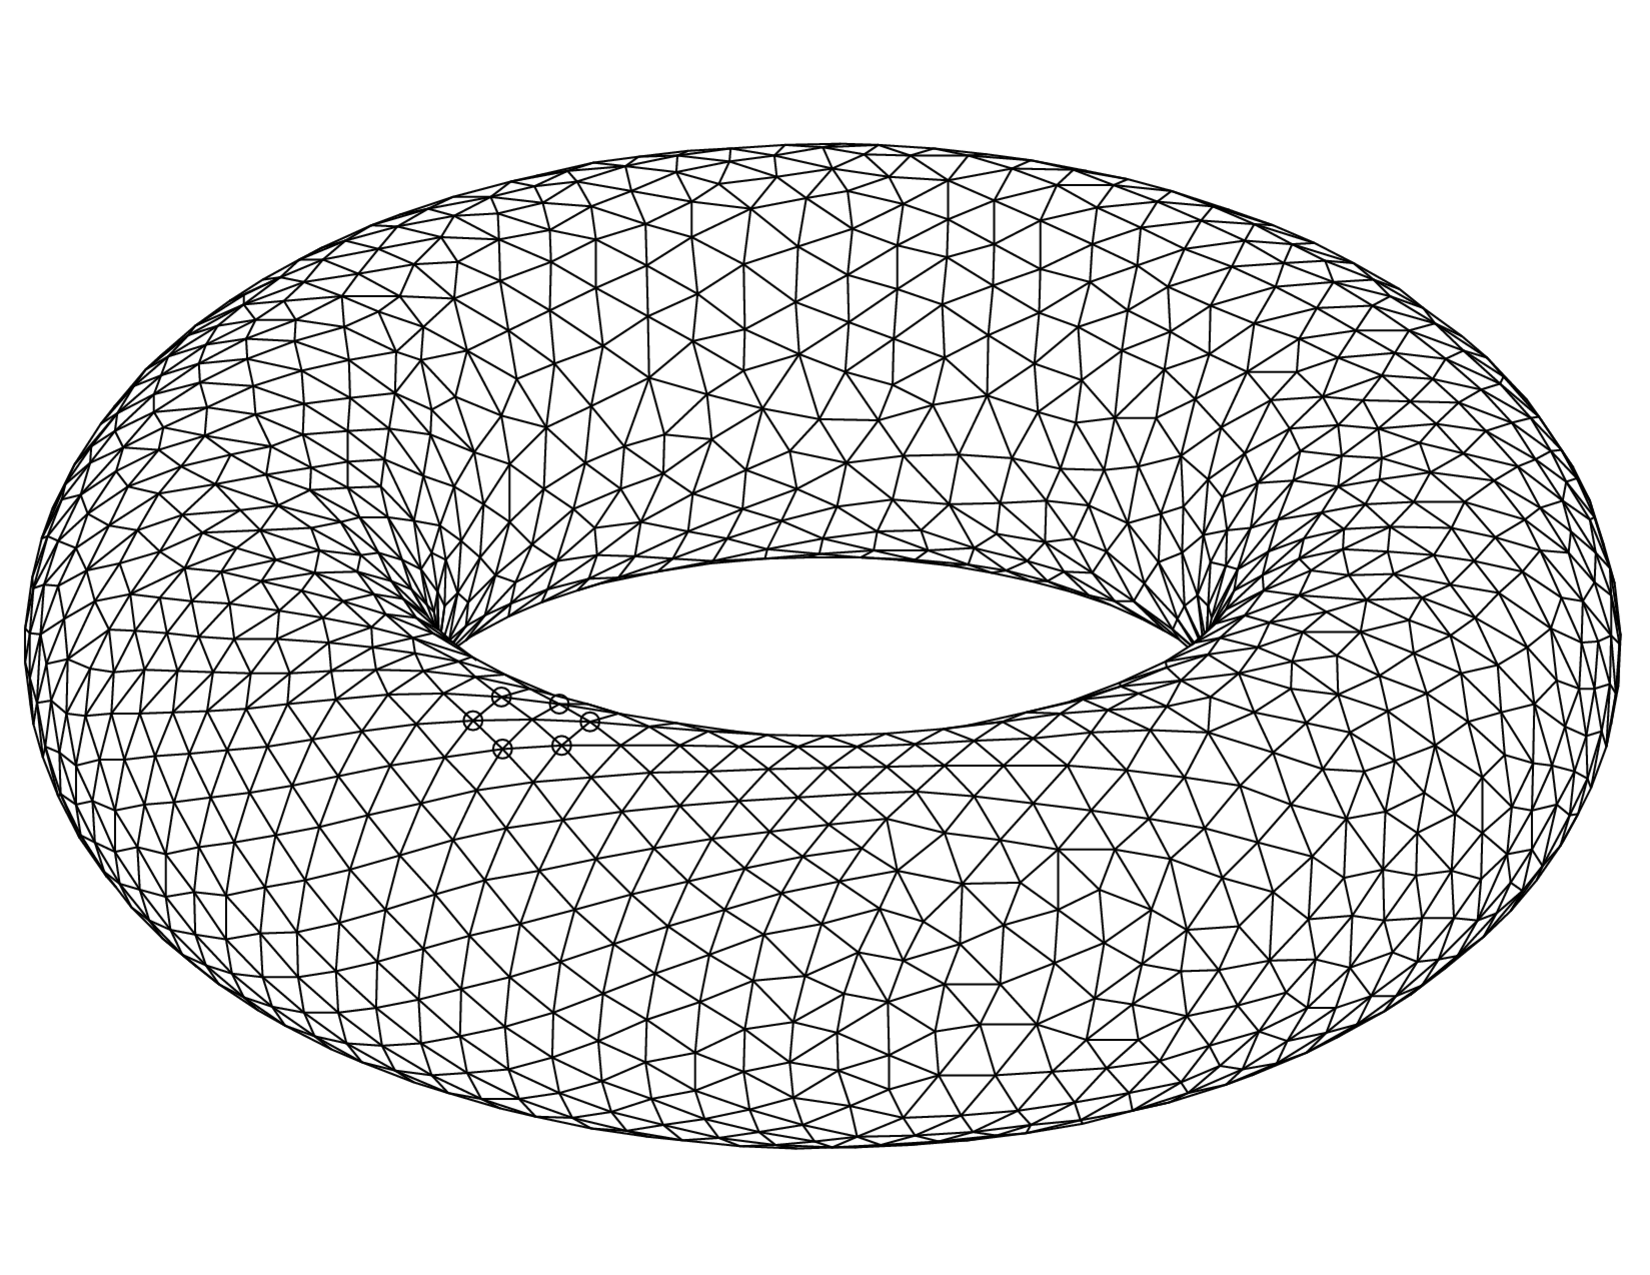
\includegraphics[width=.3\textwidth]{background/Torus-triang}
\caption{A triangulation of the torus. Image from wikipedia.}
\label{fig:triangulated-torus}
\end{figure}


